\begin{figure}[t]
  \centering
  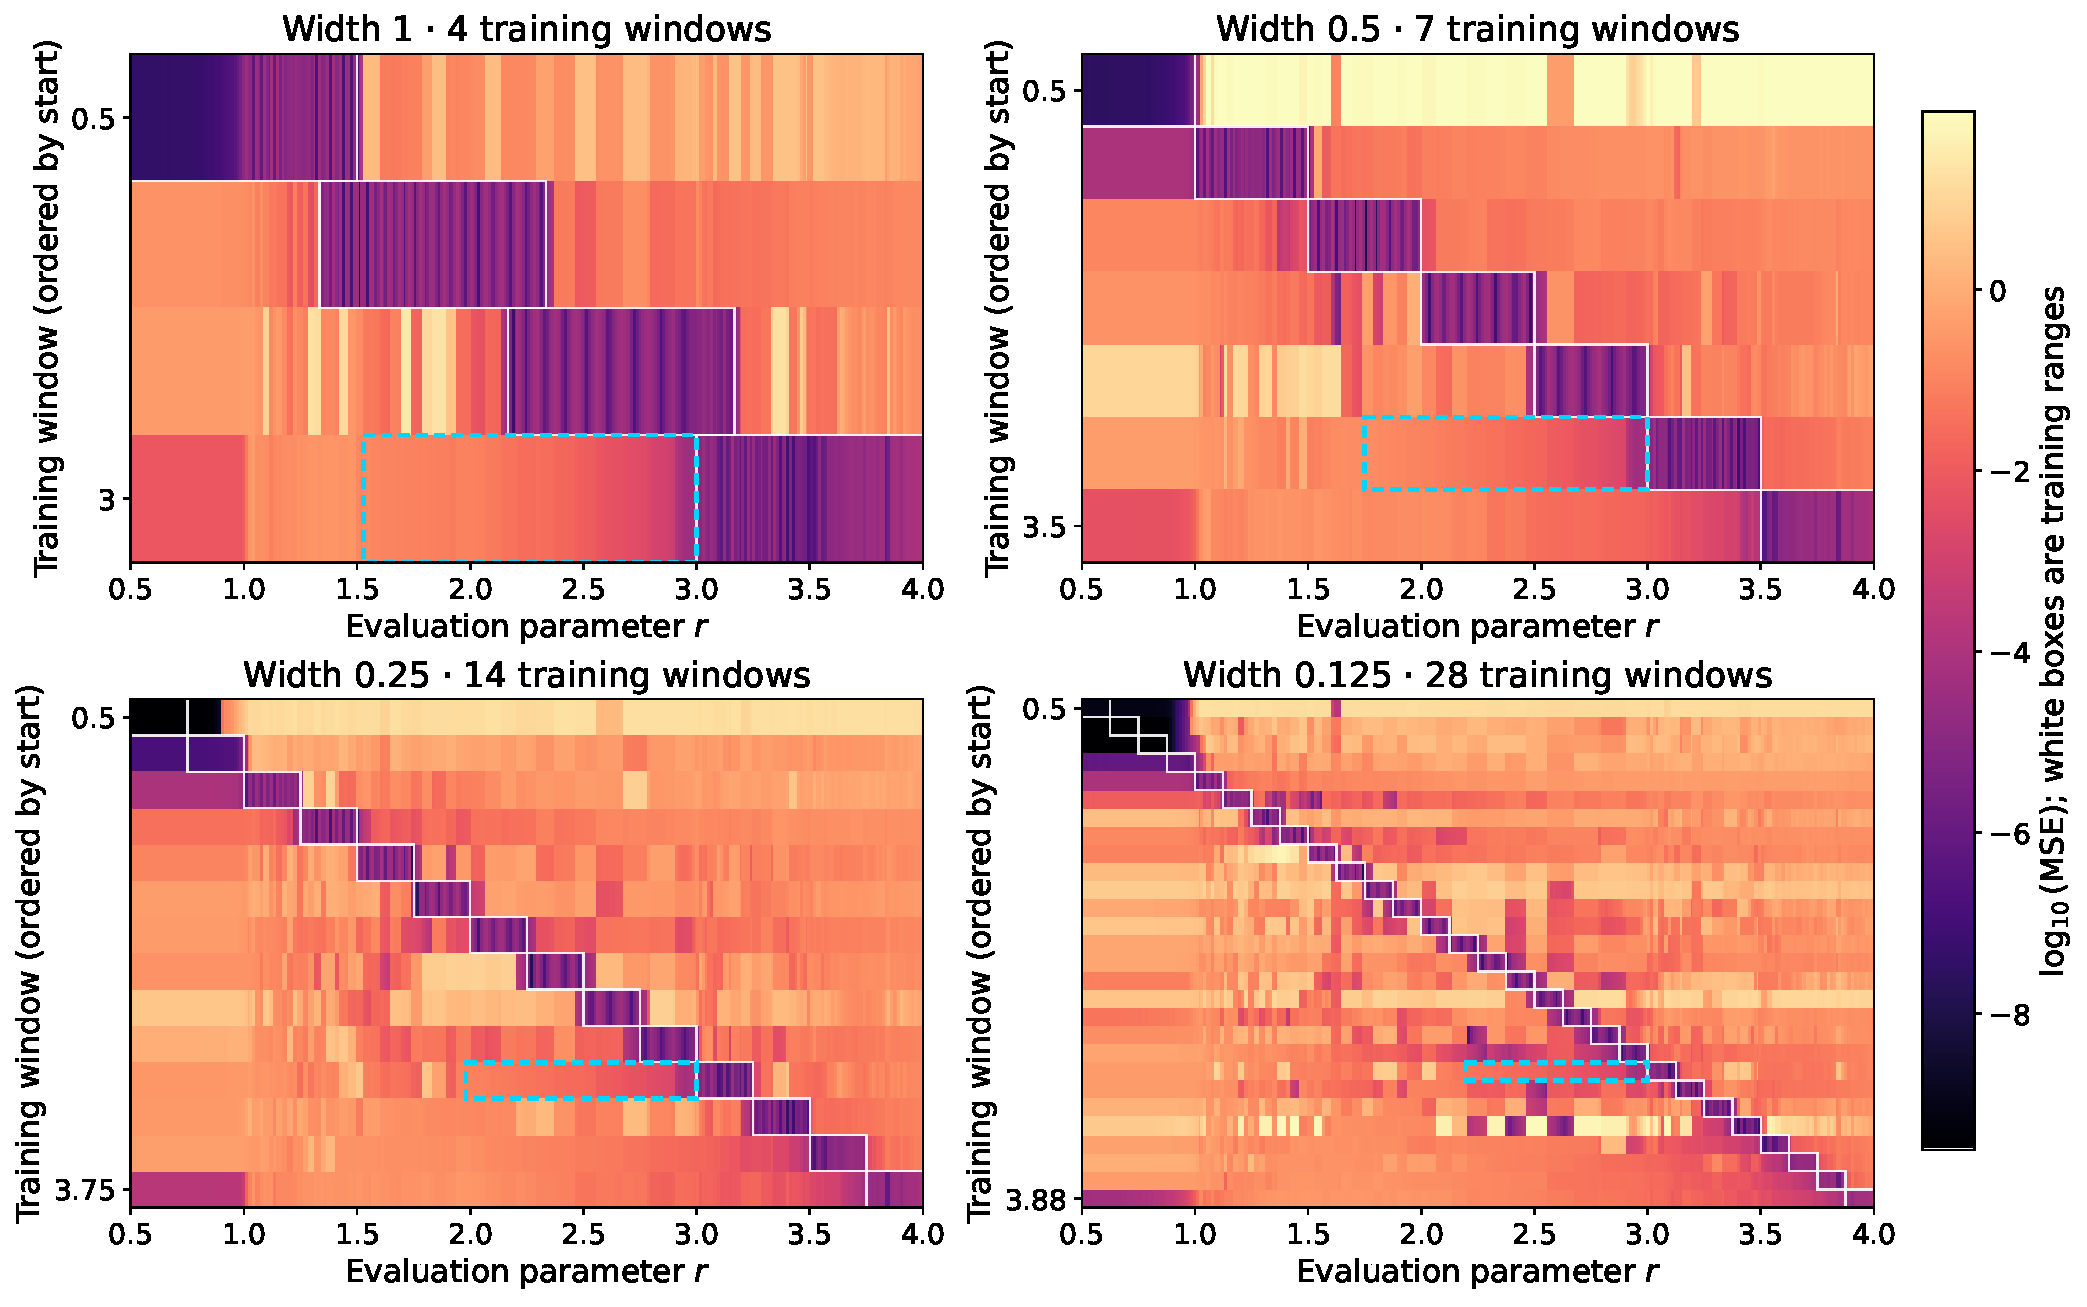
\includegraphics[width=\linewidth]{window_fixed_mse.pdf}
  \caption{\textbf{Restricted-support transfer for scalar next-state prediction.}
  Each row represents a separately trained transformer whose logistic-map
  parameters are restricted to an interval $W=[a,a+w]$; columns give the
  evaluation parameter $r\in[0.5,4]$. Panels show interval widths
  $w\in\{1,0.5,0.25,0.125\}$, corresponding to $4$, $7$, $14$, and $28$
  overlapping training windows. White rectangles mark each model's training
  interval. Color denotes the mean one-step squared error on held-out
  trajectories as $\log_{10}(\mathrm{MSE})$, using a shared scale across all
  panels (dark indicates lower error). Cyan dashed rectangles mark the interval
  $[r_{\min}(w),3]$ predicted for the model trained on $[3,3+w]$ by matching
  the stable fixed point to the lower period-two branch. Every model receives
  $8{,}000$ trajectories, $64$ input bins, and context length $L=50$, and is
  evaluated at its fixed $160$k-step checkpoint. One training seed is shown
  for each interval.}
  \label{fig:window-heatmaps-mse}
\end{figure}
